\section{Case Study and Experiments} \label{sec:casestudy}
In this section, we will study the use of the proposed on-accelerator training 
framework. With three case studies including approximate multiplier, 
overclocking and soft error that may benefit from the on-accelerator training, 
we evaluate the framework through comprehensive experiments. Finally, we present 
some general on-accelerator training experiments.

In the approximate multiplier and overclocking case studies, we experiment on the 8-bit 
fixed-point PipeCNN \cite{pipecnn_2} on Xilinx KCU1500 board. In the soft error case study, 
we experiment with an equivalent C model of PipeCNN due to the lack of 
HLS based soft error injection tools. To evaluate the training, 
we take four representative convolution neural networks including LeNet, 
AlexNet, VGG-16 and VGG-19 as the benchmark. The neural network 
benchmark is summarized in Table \ref{tab:CNN-table}. It covers networks with 
diverse sizes and the analysis can be applied to more neural networks.
\begin{table}[h]
        \centering
        \vspace{-0.3em}
        \caption{Neural network benchmark}
        \label{tab:CNN-table}
        \vspace{-0.3em}
        \begin{tabular}{c|c|c|c}
		\toprule
		  & Dataset & Layers & Total weights \\
		\midrule
		LeNet & Mnist & 4 & 60K \\
		\midrule
		AlexNet & ImageNet & 8 & 61M \\
		\midrule
		VGG-16 & ImageNet & 16 & 138M \\
		\midrule
		VGG-19 & ImageNet & 19 & 143M \\
		\bottomrule
        \end{tabular}
        \vspace{-1em}
\end{table}


\subsection{CNN accelerator with approximate arithmetic logic}
Approximate arithmetic logic that promises high-performance and energy-efficient computing has 
been studied intensively in prior work\cite{Miao_40,han_41}. When the approximate arithmetic logic 
is used in a CNN accelerator, the computing result of a neural network will be different 
from the exact computing result and lead to prediction accuracy loss when deploying 
the neural network model directly as shown in Section \ref{sec:motivation}. 
An intuitive approach is to train with software simulation, but some of the approximate arithmetic 
operators are rather complex when simulated with software i.e.\cite{appro_45}. Particularly, some of the 
approximate arithmetic unit relies on underlying semiconductor devices which 
can hardly be simulated with software i.e.\cite{appro_46}. The proposed on-accelerator 
training framework fits well with these situations. 

In this experiment, we mainly focus on the prediction accuracy loss and 
take the dynamic-range approximate multiplier proposed in \cite{Approximate_Multiplier_31} as 
an approximate computing example. The multiplier is implemented on top of the PipeCNN
accelerator. Basically, it reserves the most significant non-zero bits as well as the 
following $k$ lower bits. Larger $k$ will keep more valid digits and the multiplier 
is more accurate. On the contrast, smaller $k$ leads to lower precision but 
more efficient computing. 

Figure \ref{fig:k2-approximate-multiplier} shows the 
neural network prediction accuracy when running on the approximate CNN 
accelerator with $k=2$. According to the accuracy comparison of the models with 
offline training and on-accelerator training, it can be found that the 
top1 and top5 prediction accuracy improvement is up to 14.4\% and 16.1\% respectively. 
When $k=3$, the offline trained model accuracy is much higher due to the improved 
computing precision leaving little optimization space. The average prediction 
accuracy is still improved, though the improvement is less significant.
LeNet which is a small yet resilient network does not show much 
difference on the different training approaches and $k$ setup.
\begin{figure}
        \center
        \subfloat[top1]{
                \label{fig:appro-k2-top1}
                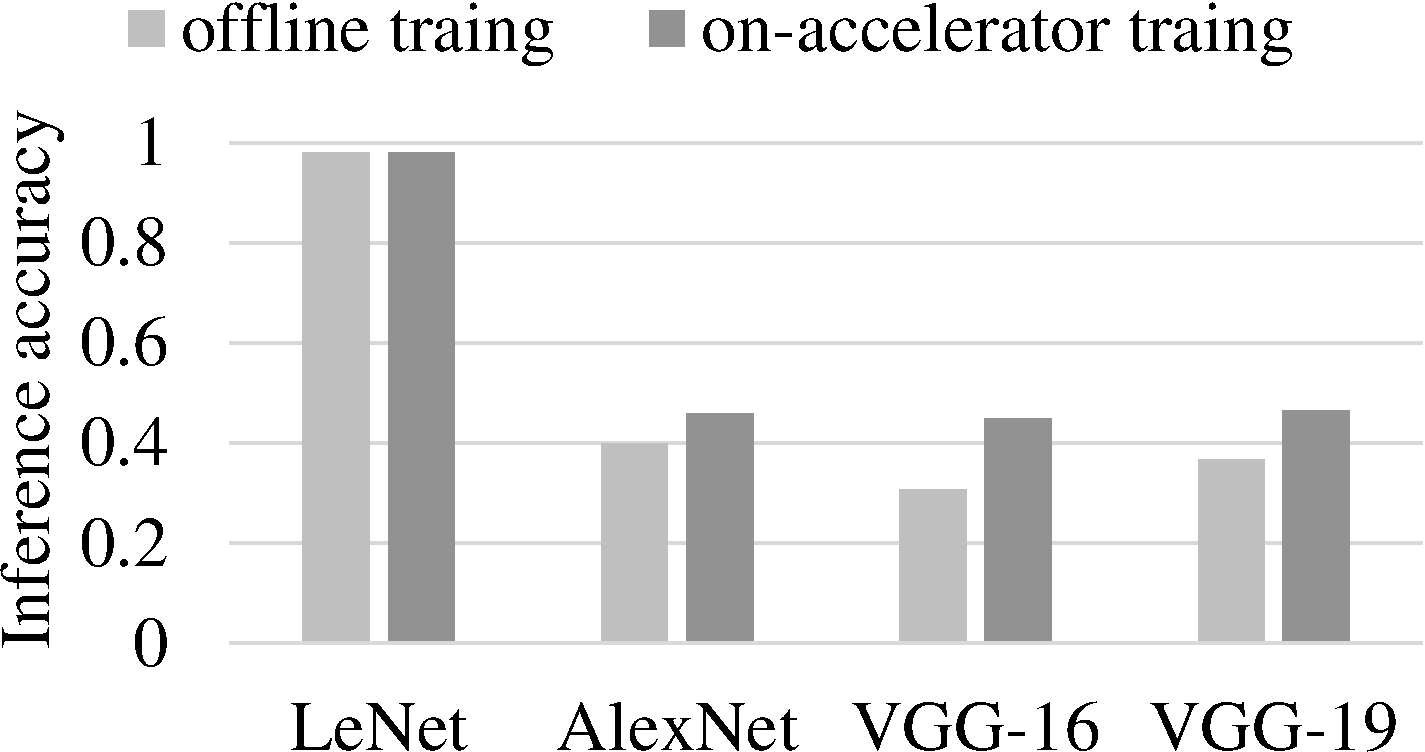
\includegraphics[width=0.65\linewidth]{appro-k2-top1}
        }
        \qquad
        \subfloat[top5]{
                \label{fig:appro-k2-top5}
                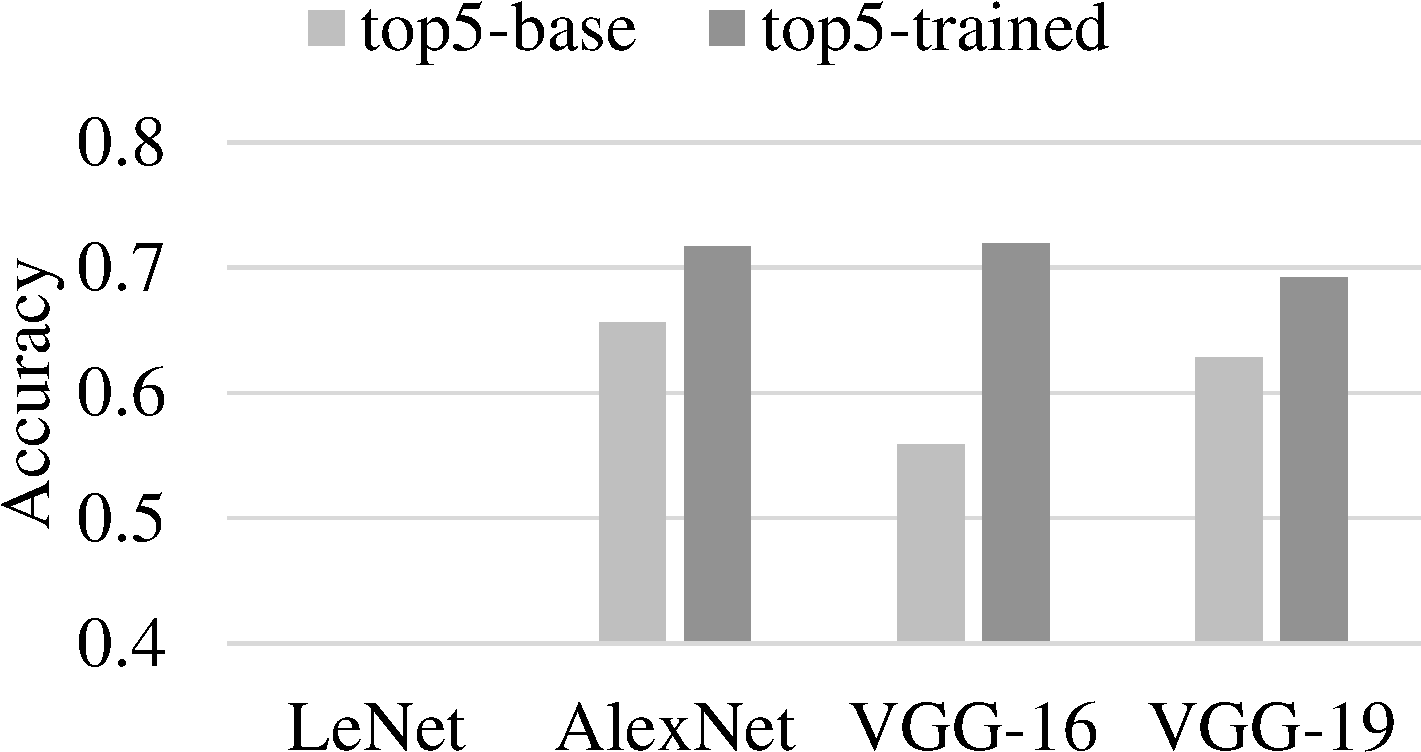
\includegraphics[width=0.65\linewidth]{appro-k2-top5}
        }
        \caption{The prediction accuracy of the neural network on accelerator with approximate multiplier(k=2)}
        \label{fig:k2-approximate-multiplier}
\end{figure}

\begin{figure}
        \center
        \subfloat[top1]{
                \label{fig:appro-k3-top1}
                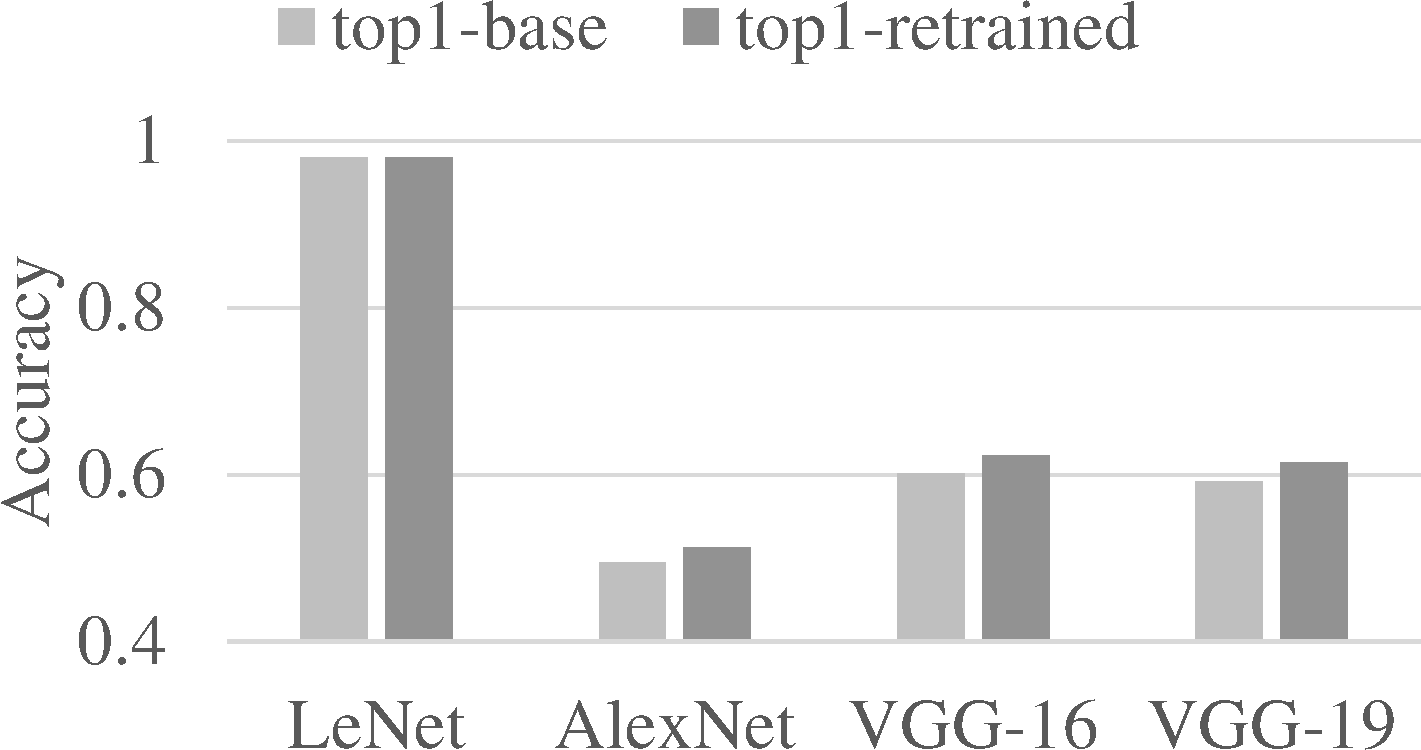
\includegraphics[width=0.6\linewidth]{appro-k3-top1}
        }
        \qquad
        \subfloat[top5]{
                \label{fig:appro-k3-top5}
                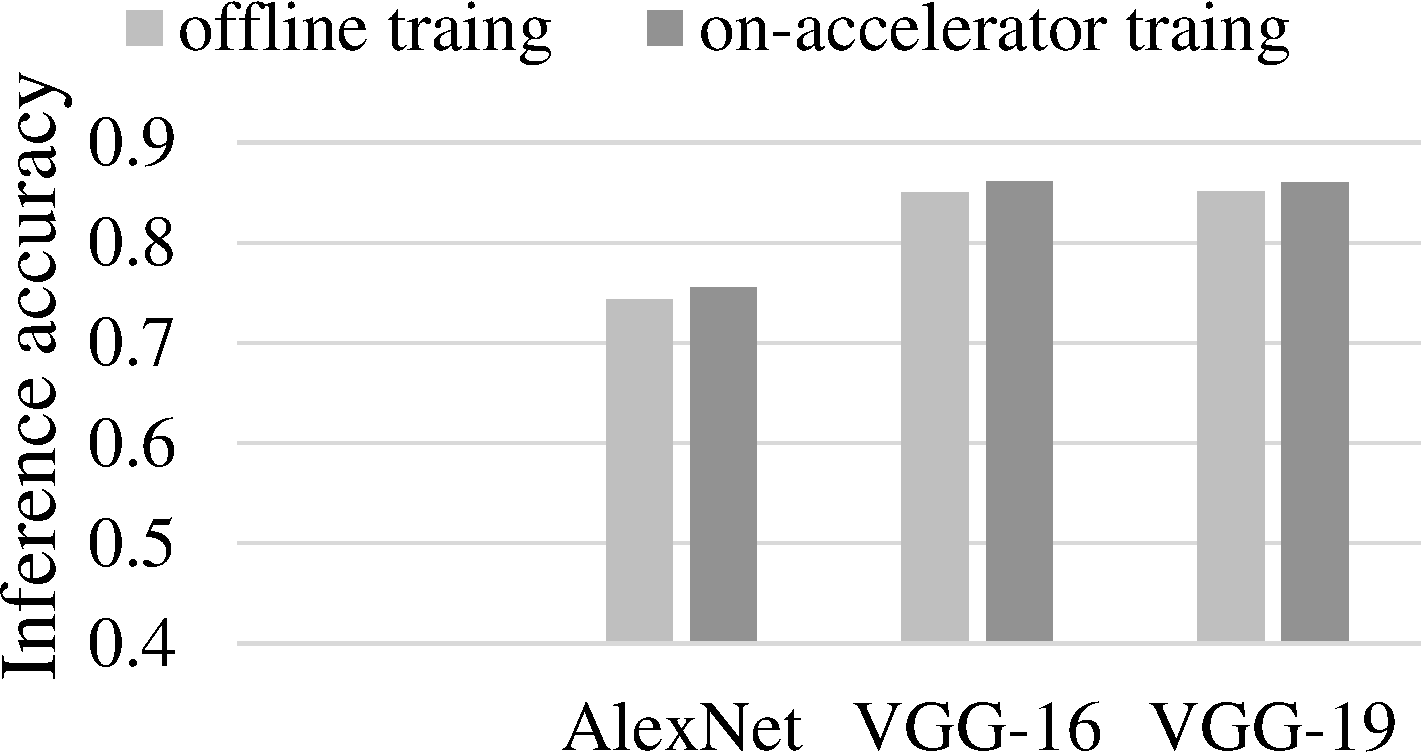
\includegraphics[width=0.6\linewidth]{appro-k3-top5}
        }
        \caption{The prediction accuracy of the neural network on accelerators with approximate multiplier(k=3)}
        \label{fig:k3-approximate-mltiplier}
\end{figure}

\subsection{CNN accelerator with overclocking}
Clock frequency is almost proportional to the performance of the CNN accelerator 
especially for large convolution operation which is typically computing bound. 
However, the circuit design tools typically adopt conservative design options 
in order to avoid the timing violations in the worst case. Overclocking enables 
higher clock frequency and performance, but timing errors may happen and affect 
the inference accuracy. The dynamic timing error caused by overclocking 
can not be captured by the offline training. In this case, we can also 
apply the on-accelerator training to have the computing errors tolerated 
by the models without redesigning the CNN accelerator.
\begin{figure}
        \center
	\subfloat[LeNet]{
		\label{fig:lenet}
		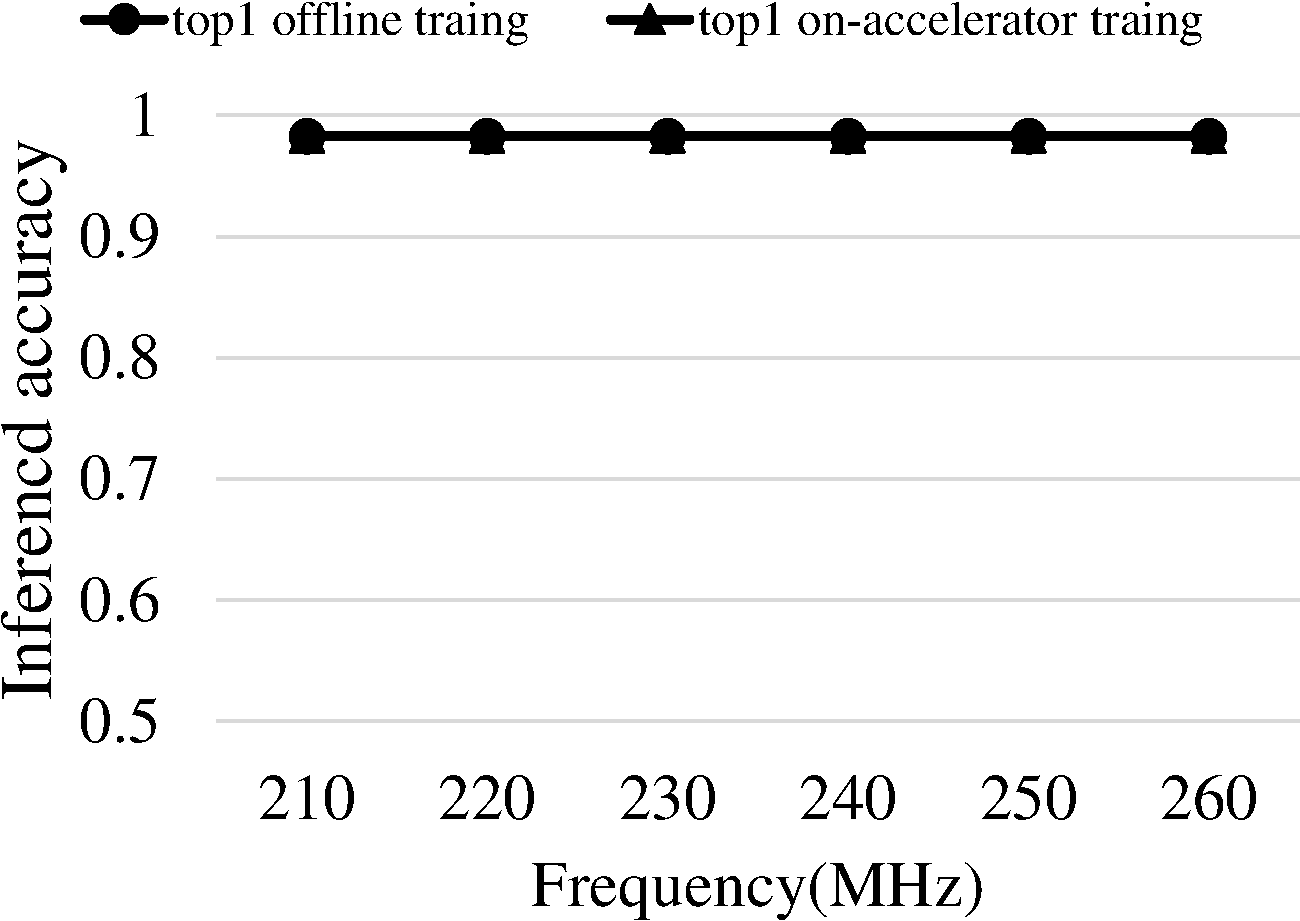
\includegraphics[width=0.6\linewidth]{lenet-overclock}
	}
	\qquad
	\subfloat[AlexNet]{
                \label{fig:alexnet}
                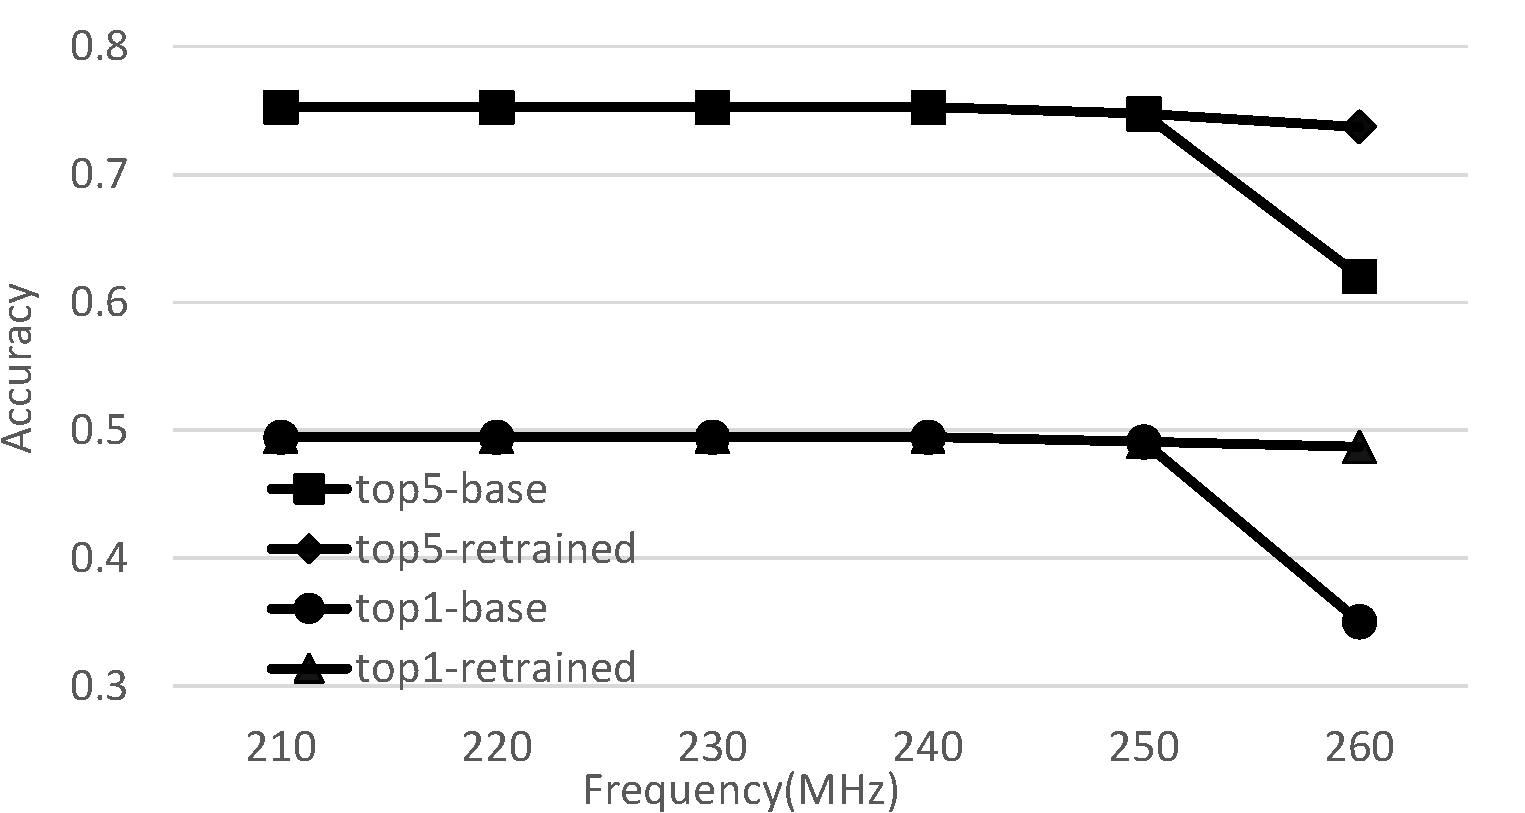
\includegraphics[width=0.6\linewidth]{alexnet-overclock}
        }
	\qquad
	\subfloat[VGG-16]{
                \label{fig:vgg16}
                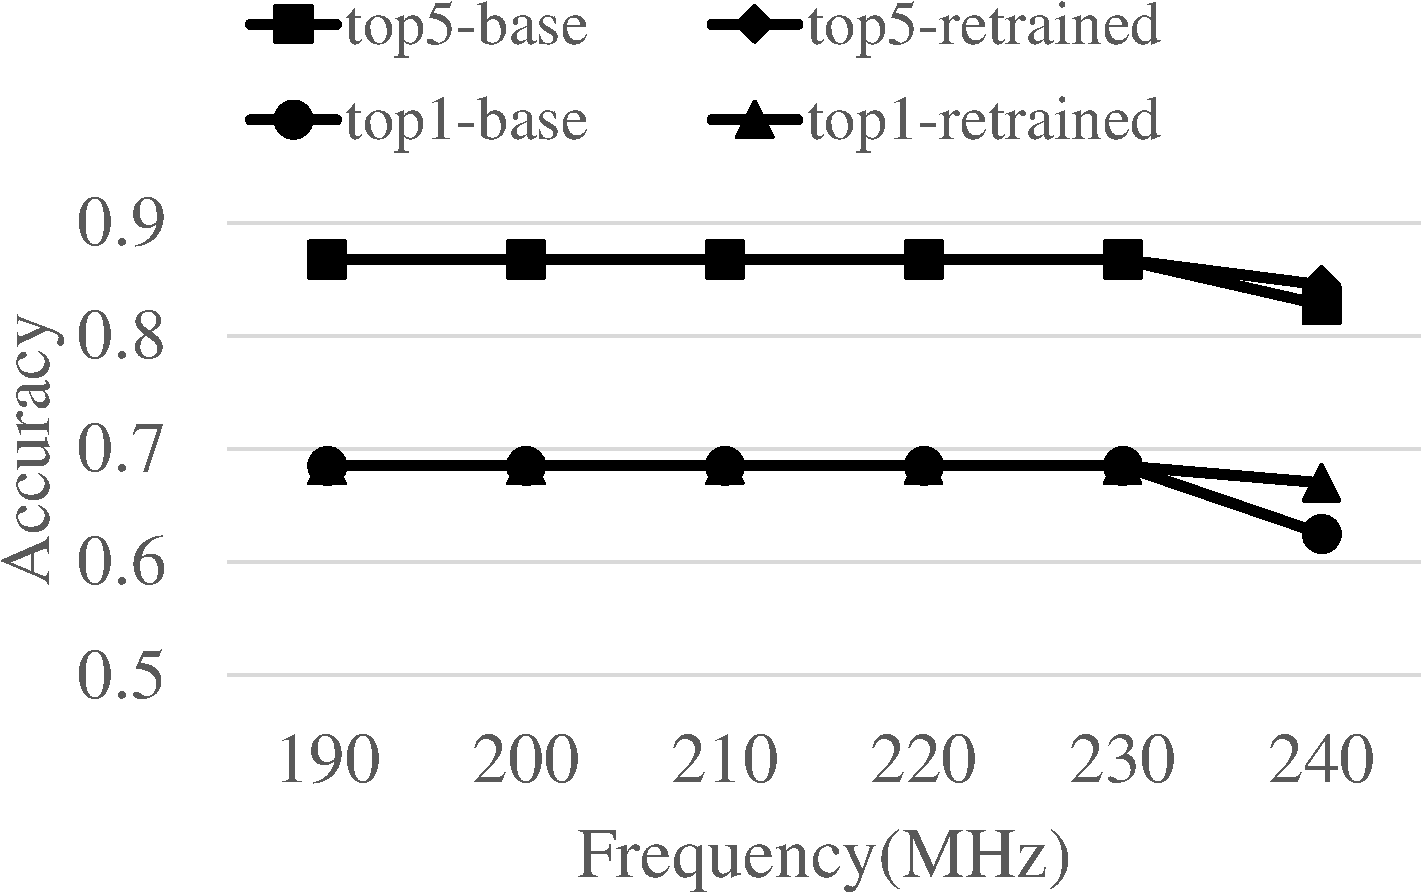
\includegraphics[width=0.6\linewidth]{vgg16-overclock}
        }
        \qquad
	\subfloat[VGG-19]{
                \label{fig:vgg19}
                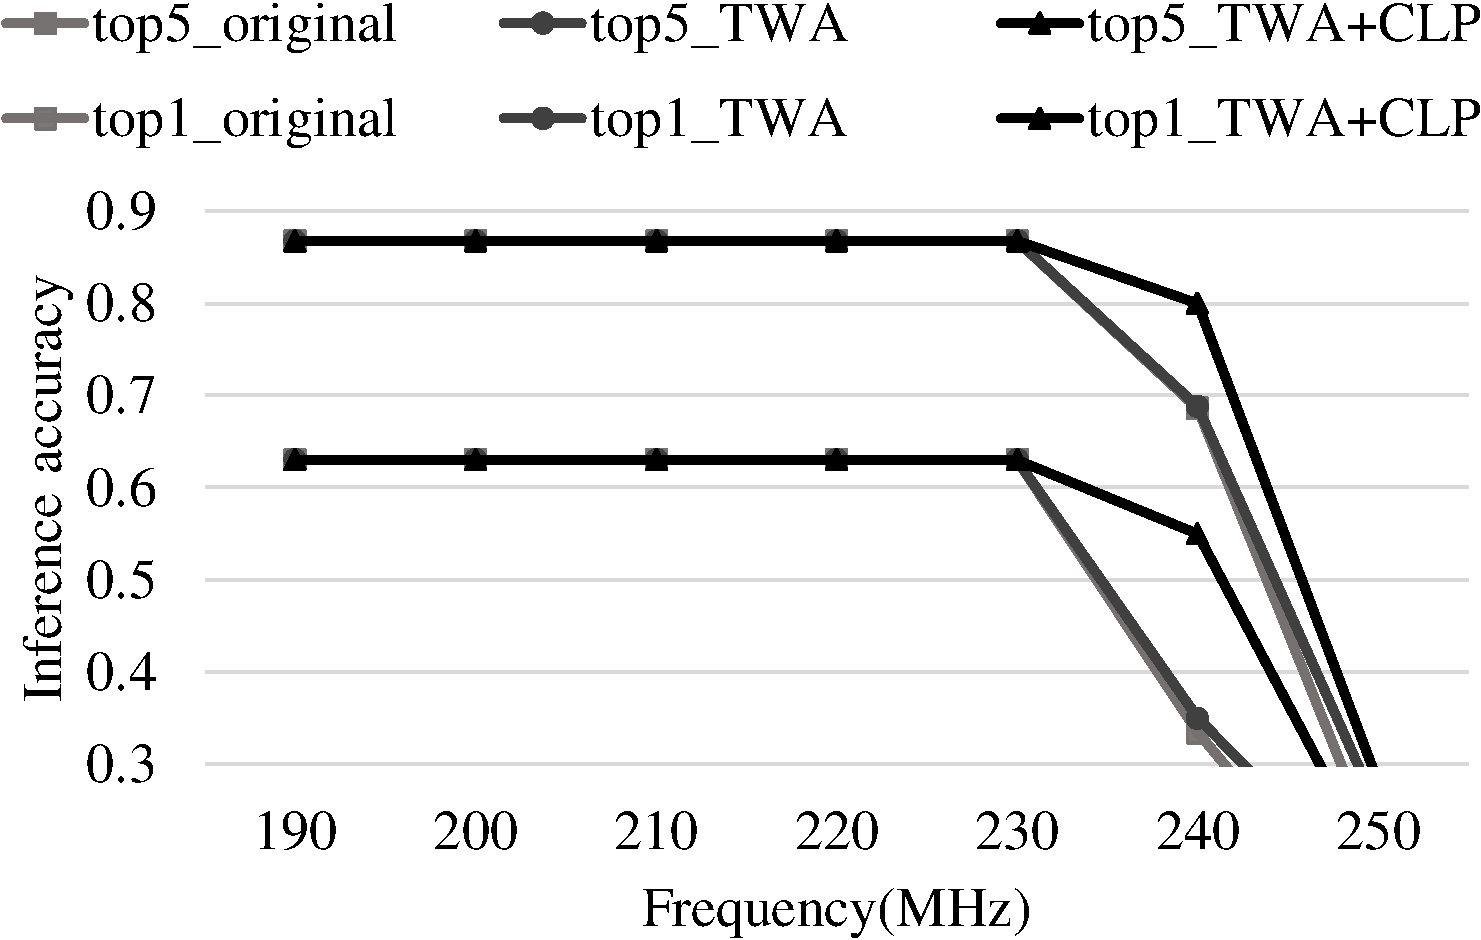
\includegraphics[width=0.6\linewidth]{vgg19-overclock}
        }
	\caption{The prediction accuracy of the benchmark neural networks on accelerators with different overclocking}
        \label{fig:overclock-accuracy}
\end{figure}


With PipeCNN, we implemented the benchmark neural networks on Xilinx KCU1500. 
LeNet and AlexNet use the same hardware implementation 
while VGG-16 and VGG-19 share the same hardware implementation. 
The two implementations work at 210 MHz and 190 MHz respectively.
With overclocking, they can be boosted to 210 MHz - 260 MHz and 
190 MHz - 240 MHz respectively. Given different overclocking frequency, 
the accelerator produces different computing results due to the variable
timing errors. It is expected that more aggressive overclocking will incur 
more computing errors and precision loss. 

On top of the overclocked CNN accelerators, we compare both the offline training and the on-accelerator training.
The prediction accuracy comparison is presented in Figure \ref{fig:overclock-accuracy}. 
Basically, the prediction accuracy will not drop until the tipping point. After the tipping point, the 
prediction accuracy degrades dramatically and can no longer be salavaged through training.
While at the extreme overclocking frequency, the on-accelerator training exhibits clear 
improvemenmt on the benchmark. Compared to the offline training, 
the on-accelerator training improves the top1 and top5 prediction accuracy 
on the extreme overclocking case by 13.7\% and 11.6\% respectively.
Compared to the original design, the clock frequency 
increases by 19\% to 26\% with small prediction accuracy loss. 
LeNet again has distinct behavior. It can tolerate all the
overclocking errors before the tipping point, but it 
also crashed given higher clock.
%  For AlexNet, VGG-16 and VGG-19, the top-5 accuracy of the retained models is improved by 3.4\%, 1.8\%, and 2\% 
%respectively at the extreme overclocking frequency. For LeNet which is a rather small yet reliable network 
%compared to the other three, the implementation remains unaffected even when the clock is boosted to 260 MHz 
%from 210 MHz. When the clock goes up to 270MHz, the timing error can no longer be tolerated by the hardware system, 
%the prediction accuracy drops to 10\% which is essentially meaningless. In this case, the base model 
%and the retrained model is pretty much the same. To ensure the stability of the overclocking experiment, 
%we also keep measuring the accuracy of the accelerators with extreme overclocking. With repeatedly 
%running the test for up to 40 hours, the measured accuracy varies slightly as present in Figure 7. 
%Despite the fact that the errors caused by the overclocking can be hardly modeled precisely at runtime, 
%the inherent error patterns may still partly be captured by the CNN model with the proposed training. 
%This explains the higher prediction accuracy with the retrained model. According to the 
%above experiments, we can conclude that the proposed accelerator aware training can produce 
%more resilient CNN model tolerating errors caused by intensive overclocking. 

%To ensure the stability of the overclocking experiment, we 
%also keep measuring the accuracy of the accelerators with extreme 
%overclocking. With repeatedly running the test for up to 40 hours, 
%the measured accuracy varies slightly as present in Figure 7. 
%Despite the fact that the errors caused by the overclocking can be 
%hardly modeled precisely at runtime, the inherent error patterns may 
%still partly be captured by the CNN model with the proposed training. 
%This explains the higher prediction accuracy with the retrained model. 
%According to the above experiments, we can conclude that the proposed 
%accelerator aware training can produce more resilient CNN model tolerating 
%errors caused by intensive overclocking. 
%
%\begin{figure}
%        \center{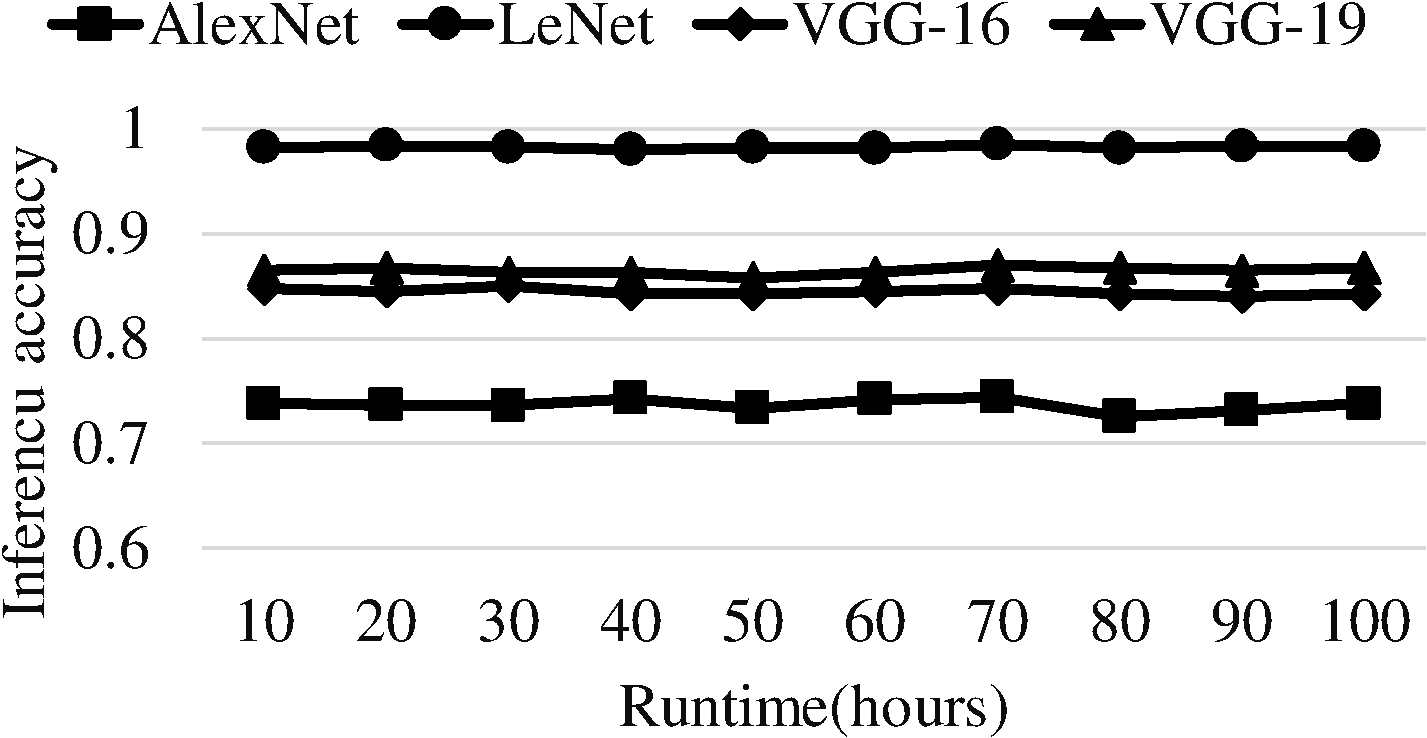
\includegraphics[width=0.6\linewidth]{stability}}
%        \caption{The Stability of Retrained Model}
%        \label{fig:stability}
%%        \vspace{-0.5em}
%\end{figure}

\subsection{CNN accelerator with soft errors}
With the shrinking semiconductor feature size and increasing FPGA capacity, 
FPGA design becomes error-prone to the soft errors. 
They can affect the behavior of the FPGA design dramatically. 
Many researchers \cite{Mansour_20,Karim_21,Nidhin_22,Subasi_23,ROSCH_24} 
have proposed various approaches to address this problem. CNN accelerators 
on FPGA can be different from the general hardware design, because 
the CNN model deployed can be further trained to tolerate the 
soft errors. As the real soft errors can hardly be modeled on GPPs, we thus
opt to adopt the on-accelerator training.

To explore the influence of soft errors on CNN accelerators, 
we need to inject soft errors to the CNN accelerators. 
In this work, we adopt a simulation-based method for the experiments. 
For the CNN accelerator, we built a C model equivalent to PipeCNN and then injected single event 
upsets (SEU) to the major components of the CNN accelerator model including the on-chip buffers 
and the computing array. With the soft error injection, we evaluate the influence of 
soft errors on the neural network prediction accuracy, The prediction accuracy 
is presented in Figure \ref{fig:softerror accuracy}. When we gradually increase the error rate, 
the prediction accuracy degrades accordingly when applying the off-line 
trained model directly on the faulty accelerators. 
%Compared to the offline training,
%the on-accelerator training improves the top1 and top5 prediction accuracy
%on the worst case by 11.1\% and 3.4\% respectively.
%When the error rate goes up to 1E-4.5, the accuracy in the worst case drops 
%by around 13.5\%. Similar to overclocking, LeNet can tolerate 
%more errors than the other three networks. The accuracy remains unchanged 
%until the error rate reaches 1E-3. When the error injection rate is low, 
%the CNN model is able to cover almost all the negative influence 
%on the prediction accuracy.

\begin{figure}
        \center
        \subfloat[LeNet]{
                \label{fig:lenet}
                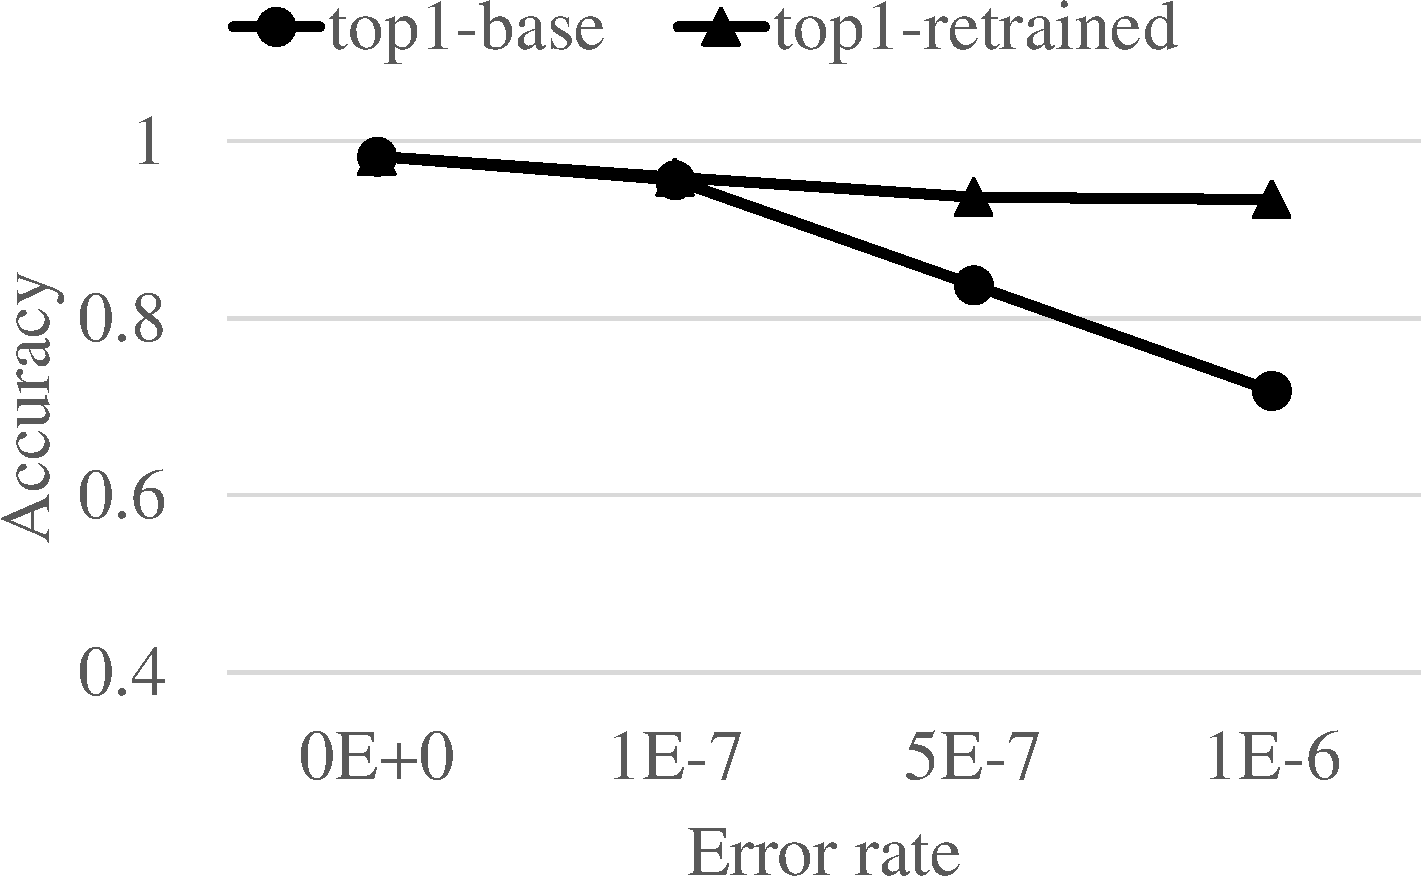
\includegraphics[width=0.6\linewidth]{lenet-softerror}
        }
        \qquad
        \subfloat[AlexNet]{
                \label{fig:alexnet}
                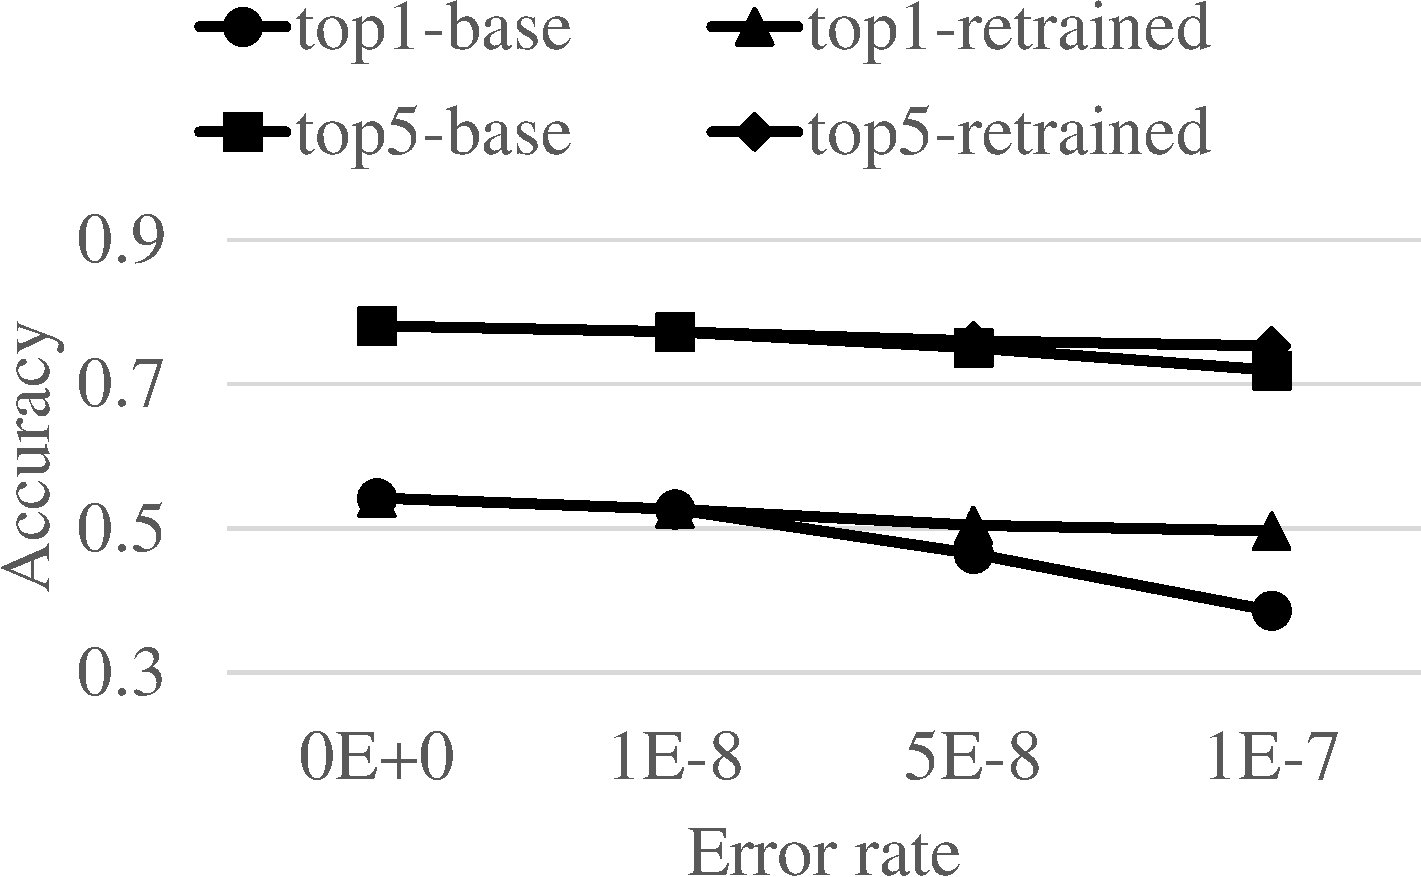
\includegraphics[width=0.6\linewidth]{alexnet-softerror}
        }
        \qquad
        \subfloat[VGG-16]{
                \label{fig:vgg16}
                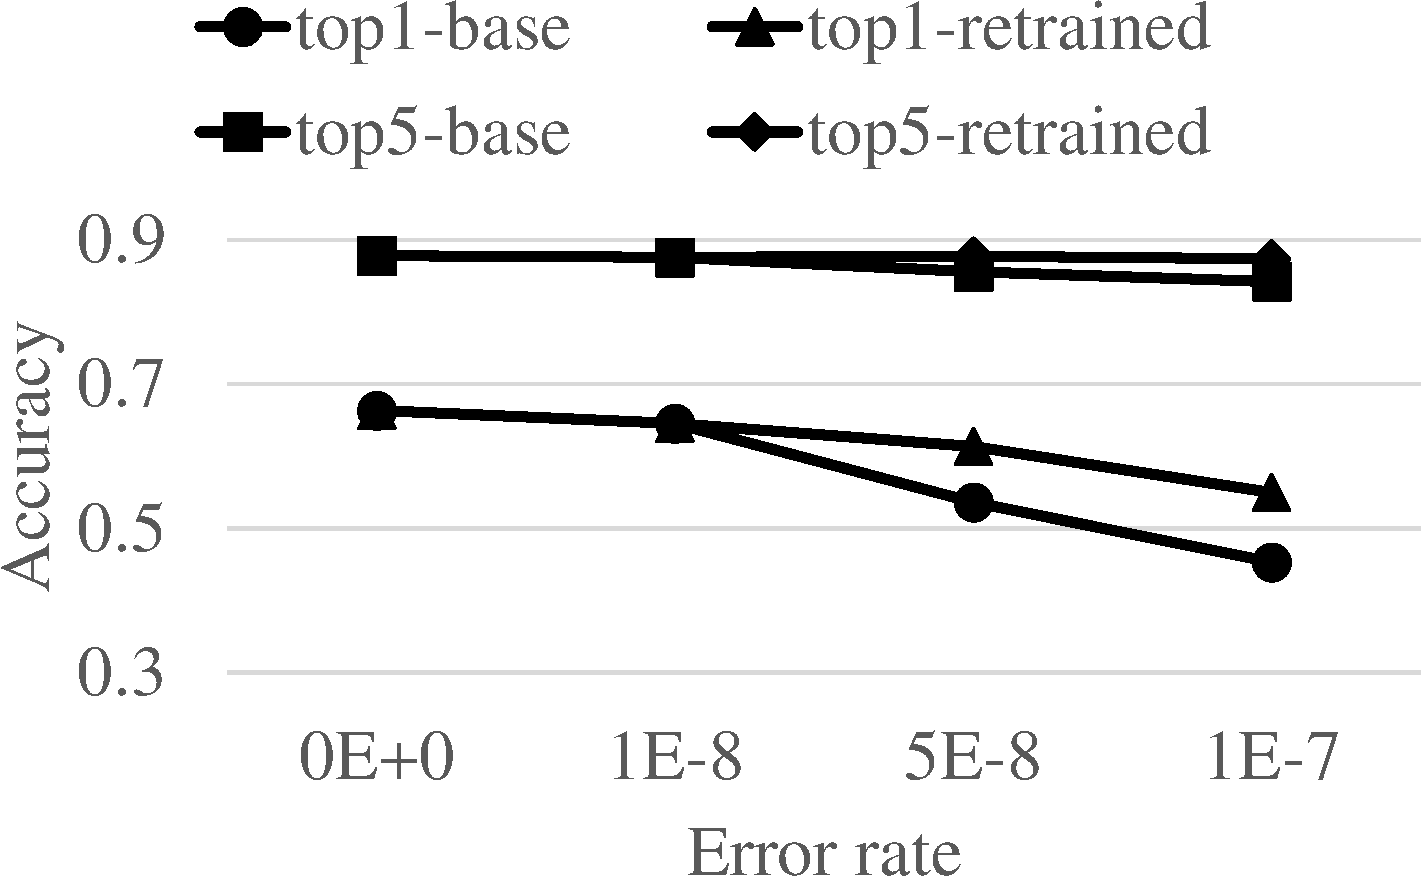
\includegraphics[width=0.6\linewidth]{vgg16-softerror}
        }
        \qquad
        \subfloat[VGG-19]{
                \label{fig:vgg19}
                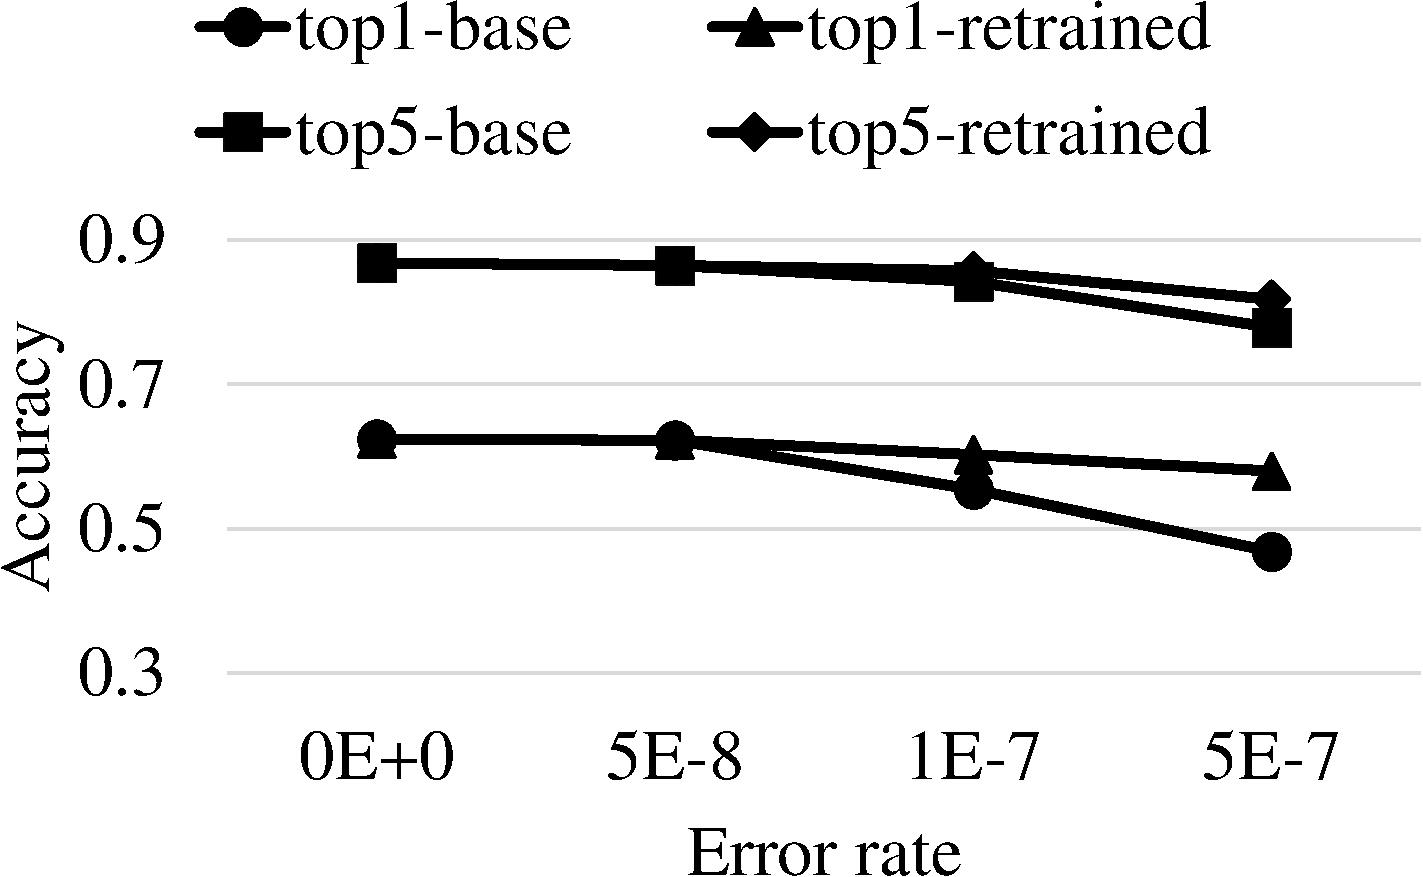
\includegraphics[width=0.6\linewidth]{vgg19-softerror}
        }
        \caption{The precision accuracy of the benchmark neural network models on accelerators with soft errors}
        \label{fig:softerror accuracy}
\end{figure}

When the error injection rate goes up, the proposed on-accelerator training becomes critical. 
According to the experiments, the top1 and top5 precision accuracy improves by 11.1\% and 3.4\%
respectively compared to the offline trained model under the highest error injection rate. 
LeNet can also tolerate higher error injection rate and exhibits the unique fault-tolerant capability.
In summary, the experiments demonstrate that we can have the CNN model to learn 
both the characteristics of the data and the underlying computing errors of the accelerator 
together using the on-accelerator training framework. The resulting CNN model becomes more resilient 
without any modification to the CNN accelerators.  

\subsection{General on-accelerator training analysis}
We also present the training time on the hybrid CPU-FPGA architecture. 
It can be seen that the training is much slower than the fixed-point training on CPU. 
This is mainly caused by the frequently data transferring between device memory and host 
memory as well as the large amount of data type converting, This will be optimized 
in our future work. In addition, it can be found that the 
training on larger network takes longer time and higher clock frequency 
is beneficial to the training time as expected.  

\begin{figure}
        \center{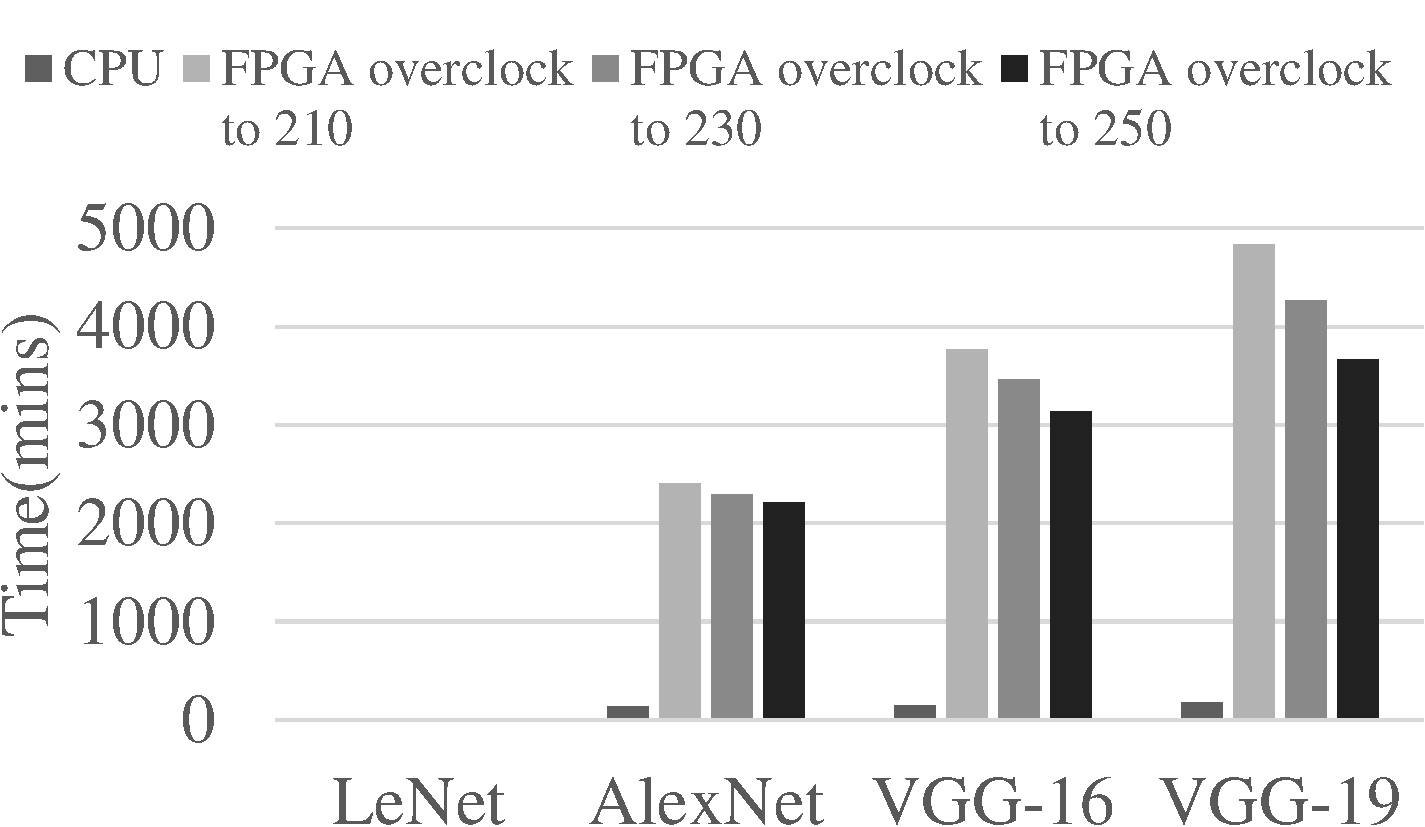
\includegraphics[width=0.6\linewidth]{time}}
        \caption{Training time}
        \label{fig:time}
%        \vspace{-0.5em}
\end{figure}


For the on-accelerator training approach, we notice that batch size is 
a critical hyper parameter. We use AlexNet as an example and show the influence of batch on the resulting model 
prediction accuracy. The result is presented in Figure \ref{fig:batch}.
According to the figure, the batch size affects the training precision clearly.
Given larger batch size, the model prediction accuracy 
increase gradually. The main reason is that larger batch training helps to 
reduce the influence of the computing error. Therefore, larger batch size is 
recommended for the on-accelerator training.

\begin{figure}
        \center{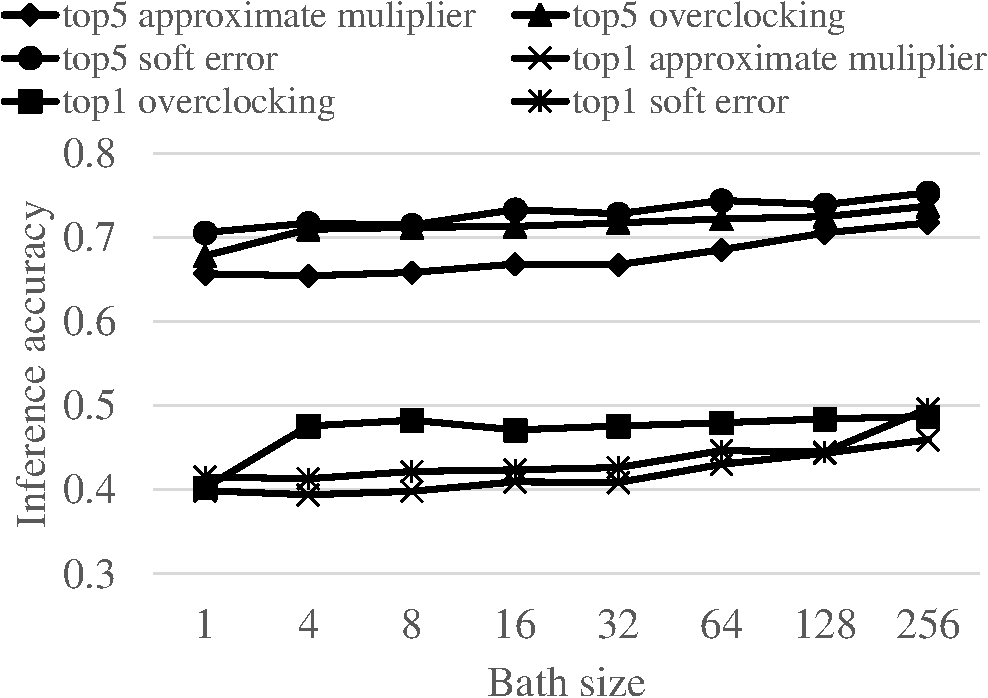
\includegraphics[width=0.6\linewidth]{batch}}
        \caption{The influence of batch size on the on-accelerator training}
        \label{fig:batch}
\end{figure}
